\chapter{Introduction}

Industrial robots have become an inseparable part of the manufacturing process in large enterprises. In small to medium-sized enterprises (SMEs), the adoption of robots has been slower, mainly due to high entry costs and difficult reprogramming. Having the ability to quickly and easily reprogram industrial robots would accelerate their adoption in SMEs, and allow them to be used in more flexible scenarios. The ARCOR2 system~\cite{kapinus2023arcor2}, along with the Android application, AREditor, aims to streamline the reprogramming process by utilizing augmented reality and a tablet device.  The options for setting a pose of the robot from the app are, however, limited, hindering its usability. 

When programming robots in AREditor, the user uses the robot arm to define points in space. When working with collaborative robots, the operator can reposition the robot manually -- by grabbing the robot arm and dragging it to the desired spot. This task becomes more tedious when the robot cannot be moved by hand. AREditor provides incremental stepping functionality, allowing the user to move the robot arm by selected increment in the direction of a chosen axis. This is sufficient for minor tweaking and fine-tuning but becomes too slow when a more substantial repositioning is necessary. Another problem is the lack of visualization of the final pose. 

This thesis proposes a novel system for rapid positioning of a robot, employing a model robot rendered on-screen over the real robot in the workspace. Through this approach, the user can directly manipulate the model without affecting the robot, which allows for a safe interaction, unconstrained by the movement speed limit of the particular robot. Another benefit to this approach is the ability to visualize different poses before committing to a final one, thus saving time repositioning. 

The thesis is structured as follows: in the first chapter, a brief summary of related research is presented. The second chapter contains a rundown of the ARCOR2 system and the related user interface AREditor. In the following chapters, the design and implementation of the final system is described. Finally, the realized user testing is presented and evaluated. 

\chapter{Related Work}
With rising interest in industrial robots, simplification of robot programming has been at the forefront for many researchers. Suzuki et al.\cite{suzuki2022augmented} compiled 460 papers on AR-enabled human-robot interaction (AR-HRI), categorizing the works into various categories. The survey has shown that most research is focused on facilitating programming and supporting real-time control. When it comes to devices, however, most researchers favor on-body, wearable devices (especially head-mounted displays) over handhelds. 

\section{Wearable devices}
Head-mounted displays (HMDs) provide an immersive experience and free up the hands of the operator, allowing them to perform work while always having crucial information in their field of vision. However, the lack of a tangible device in the hands of the user begets a question of how they will interact with the workplace. Popular approaches include gestures \cite{voicelargescale, handsfree, packing}, handheld pointers \cite{2009, speared}, and less commonly voice commands \cite{voicelargescale}. Park et al.\cite{handsfree} propose a hands-free system utilizing head gestures and gaze for selection and interaction. Chan et al.\cite{voicelargescale} created an interface allowing the user to set trajectory points on the work surface using a combination of gaze and voice commands. Ong et al.\cite{ONG2020101820} combines a stereoscopic HMD with a physical handheld pointer, representing the end-effector. In this instance, the display is created by combining a VR headset and two webcams mounted directly onto it. A much more prevalent approach is to use an AR headset, such as the Microsoft HoloLens. The SPEARED framework by Yigitbas et al.\cite{speared} uses the HoloLens to display the current robot working state and detected objects, but also the current program in the form of code blocks, which can be modified in the AR environment. In the case of SPEARED, there is no direct robot pose manipulation, all interaction is conducted through code. Chan et al.\cite{voicelargescale} also utilizes the Microsoft HoloLens, but allows the user to directly set trajectories by using a combination of gaze and voice commands. 


\section{Handheld devices}

While there have been works focusing on AR-enabled robot programming systems for handheld devices, they certainly represent a minority, especially concerning direct robot pose manipulation. The interface often only allows the user to program 'pick and place' tasks, or the robot is programmed kinesthetically\cite{picknplace, Tango}.

Pertaining to controlling the robot pose explicitly, two main approaches can be discerned: individual joint setting and end effector location setting. Setting each joint rotation individually is not suitable for end-users lacking experience with robotics, and even skilled operators rarely utilize it. Most implementations, however, provide both options. An earlier work by Frank et al.\cite{planar} developed a system for controlling a planar robot on a tablet device, which provides the user with the ability to control both end effector location and individual angles through tapping and dragging on the screen. Zhang et al.\cite{ZHANG20201221} provide the user with a set of arrows to control each joint separately, or to command the end effector directly, with a similar approach being taken in some older works\cite{pendant}. 



\chapter{ARCOR2}
ARCOR2 (Augmented Reality Collaborative Robot) is a framework for visual programming of industrial robots developed by the research group Robo@FIT. It enables end-users to create programs by defining points in space and program steps, which are spatially visualized, allowing for an easy understanding of work processes. The system can generate code from visually defined procedures and facilitates control of its execution. Multiple robots, machines, and services can be included in a single workspace, with multiple concurrent users to be connected. New robots and services can be integrated by implementing an \texttt{Object Type} -- a plugin into the system representing an interface between ARCOR2 and a real-world object, e.g. a type of robot~\cite{kapinus2023arcor2}.

The system is divided into backend, comprising several independent services, and frontend (in this case, AREditor)~\cite{arcor2}. The main service handling all incoming and outgoing communication is ARServer. ARServer is in charge of propagating messages to other services, holding system state, and sending out notifications upon changes. UIs such as AREditor can interact with the system state through RPCs.

\section{API}
Communication between ARServer and AREditor takes place through WebSockets. The communication protocol is based on RPCs and events, which are defined in the form of dataclasses\footnote{\url{https://docs.python.org/3/library/dataclasses.html}} and serialized into JSON \myworries{this is word for word, change?}. 

Dataclasses are used to create an OpenAPI\footnote{\href{https://www.openapis.org/}{https://www.openapis.org/}} representation, which is subsequently used to generate C\# classes used in AREditor. In AREditor, each RPC is represented by such class in the \texttt{IO.Swagger.Model} namespace, and contains a method to serialize self to JSON.

\subsection{RPCs}
To each RPC (Remote Procedure Call) sent by AREditor, the server elicits a response. The response contains the resulting data. If the request fails, the data field is empty, and a message informing of the error. An example of a successful request-response sequence would be: 
\begin{verbatim}
    RPC request: 
    InverseKinematics.Request(
        id=28, 
        request='InverseKinematics', 
        args=InverseKinematics.Request.Args(
            robot_id='obj_edc94797032d410289f7cd241b5c6fe8', 
            end_effector_id='default', 
            pose=Pose(...), 
            start_joints=[...], 
            avoid_collisions=True, 
            arm_id=None)) 
    
    RPC response:
        InverseKinematics.Response(
            id=28, 
            response='InverseKinematics', 
            result=True, 
            messages=None, 
            data=[...])
\end{verbatim}

Note that the result field is true, and there is no message. Had the request failed, the response would look as follows:

\begin{verbatim}
     RPC response:
        InverseKinematics.Response(
            id=29, 
            response='InverseKinematics', 
            result=False, 
            messages=['arcor2 (General): Failed to compute IK.'], 
            data=None)
\end{verbatim}

\subsection{Events}
The main purpose of events is to notify connected user interfaces of asynchronous events. Notifications are frequently sent after an RPC has been processed. The pattern then becomes:
\begin{enumerate}
    \item RPC request
    \item RPC processed; response sent
    \item Event broadcasted
\end{enumerate}

A typical use case can be observed in robot stepping. User sends a request to move the end-effector, the end-effector is moved, and after the movement is finished, an event is sent to notify AREditor and all other connected user interfaces of the changed robot pose.

\section{AREditor}
AREditor is a mobile application used to interface with ARCOR2. AREditor aims to allow users with little or no programming experience to create programs within the workspace. Within the application, users can easily interact with the robotic workspace through augmented reality. 

After connecting to ARServer, the user is presented with the main screen, from where he can create or open scenes, projects, and packages. When a scene (project, package) is opened, the application switches to the editor.

\subsection{Architecture}

AREditor comprises several singleton classes handling the most important functionality such as communication with ARServer, holding the application state, and managing the current open scene or project. They provide events, to which the individual screens and menus can dynamically subscribe.

\subsubsection{\texttt{GameManager}}

\texttt{GameManager} is the main controller of the application. It manages different screens, holds the application state, holds the connection status, and notifies users of changes. Connection to ARServer is created here, using \texttt{WebsocketManager}. 

\subsubsection{\texttt{WebsocketManager}}

The \texttt{WebsocketManager} class in AREditor is responsible for communication with ARServer. It provides methods to create connection, creates and sends RPCs, holds the websocket context, processes received data and broadcasts events, informing subscribers of changes on connection status, robot pose, action objects addition/removal, etc. 

For outgoing data, each RPC request type is represented by a class, generated by OpenAPI Generator CLI\footnote{\href{https://openapi-generator.tech/}{https://openapi-generator.tech/}}. The class is instantiated, the data is serialized and sent through the websocket. Response data is awaited and deserialized using either a corresponding class, or an anonymous type\footnote{\href{https://learn.microsoft.com/en-us/dotnet/csharp/fundamentals/types/anonymous-types}{https://learn.microsoft.com/en-us/dotnet/csharp/fundamentals/types/anonymous-types}} and based on the \texttt{@event} value, the corresponding event is dispatched. 

\subsection{Editor screen}
The editor is the AR-enabled part of the application, responsible for all 3D visualization and interaction \myworries{almost word for word, should I cite?}. Available menus are listed on the left side of the screen, organized into groups, and accessible through tabs: Favorites, Add, Utility, Home, and Robot. The right side of the screen is occupied by the selector menu by default, which provides a list of action objects in the workspace. When a different menu is selected from the list, the selector menu is hidden and replaced by the corresponding menu, as pictured in \ref{fig:EditorMenus}. 

\begin{figure}
    \centering
    
        \subfloat[Selector menu, the default.]{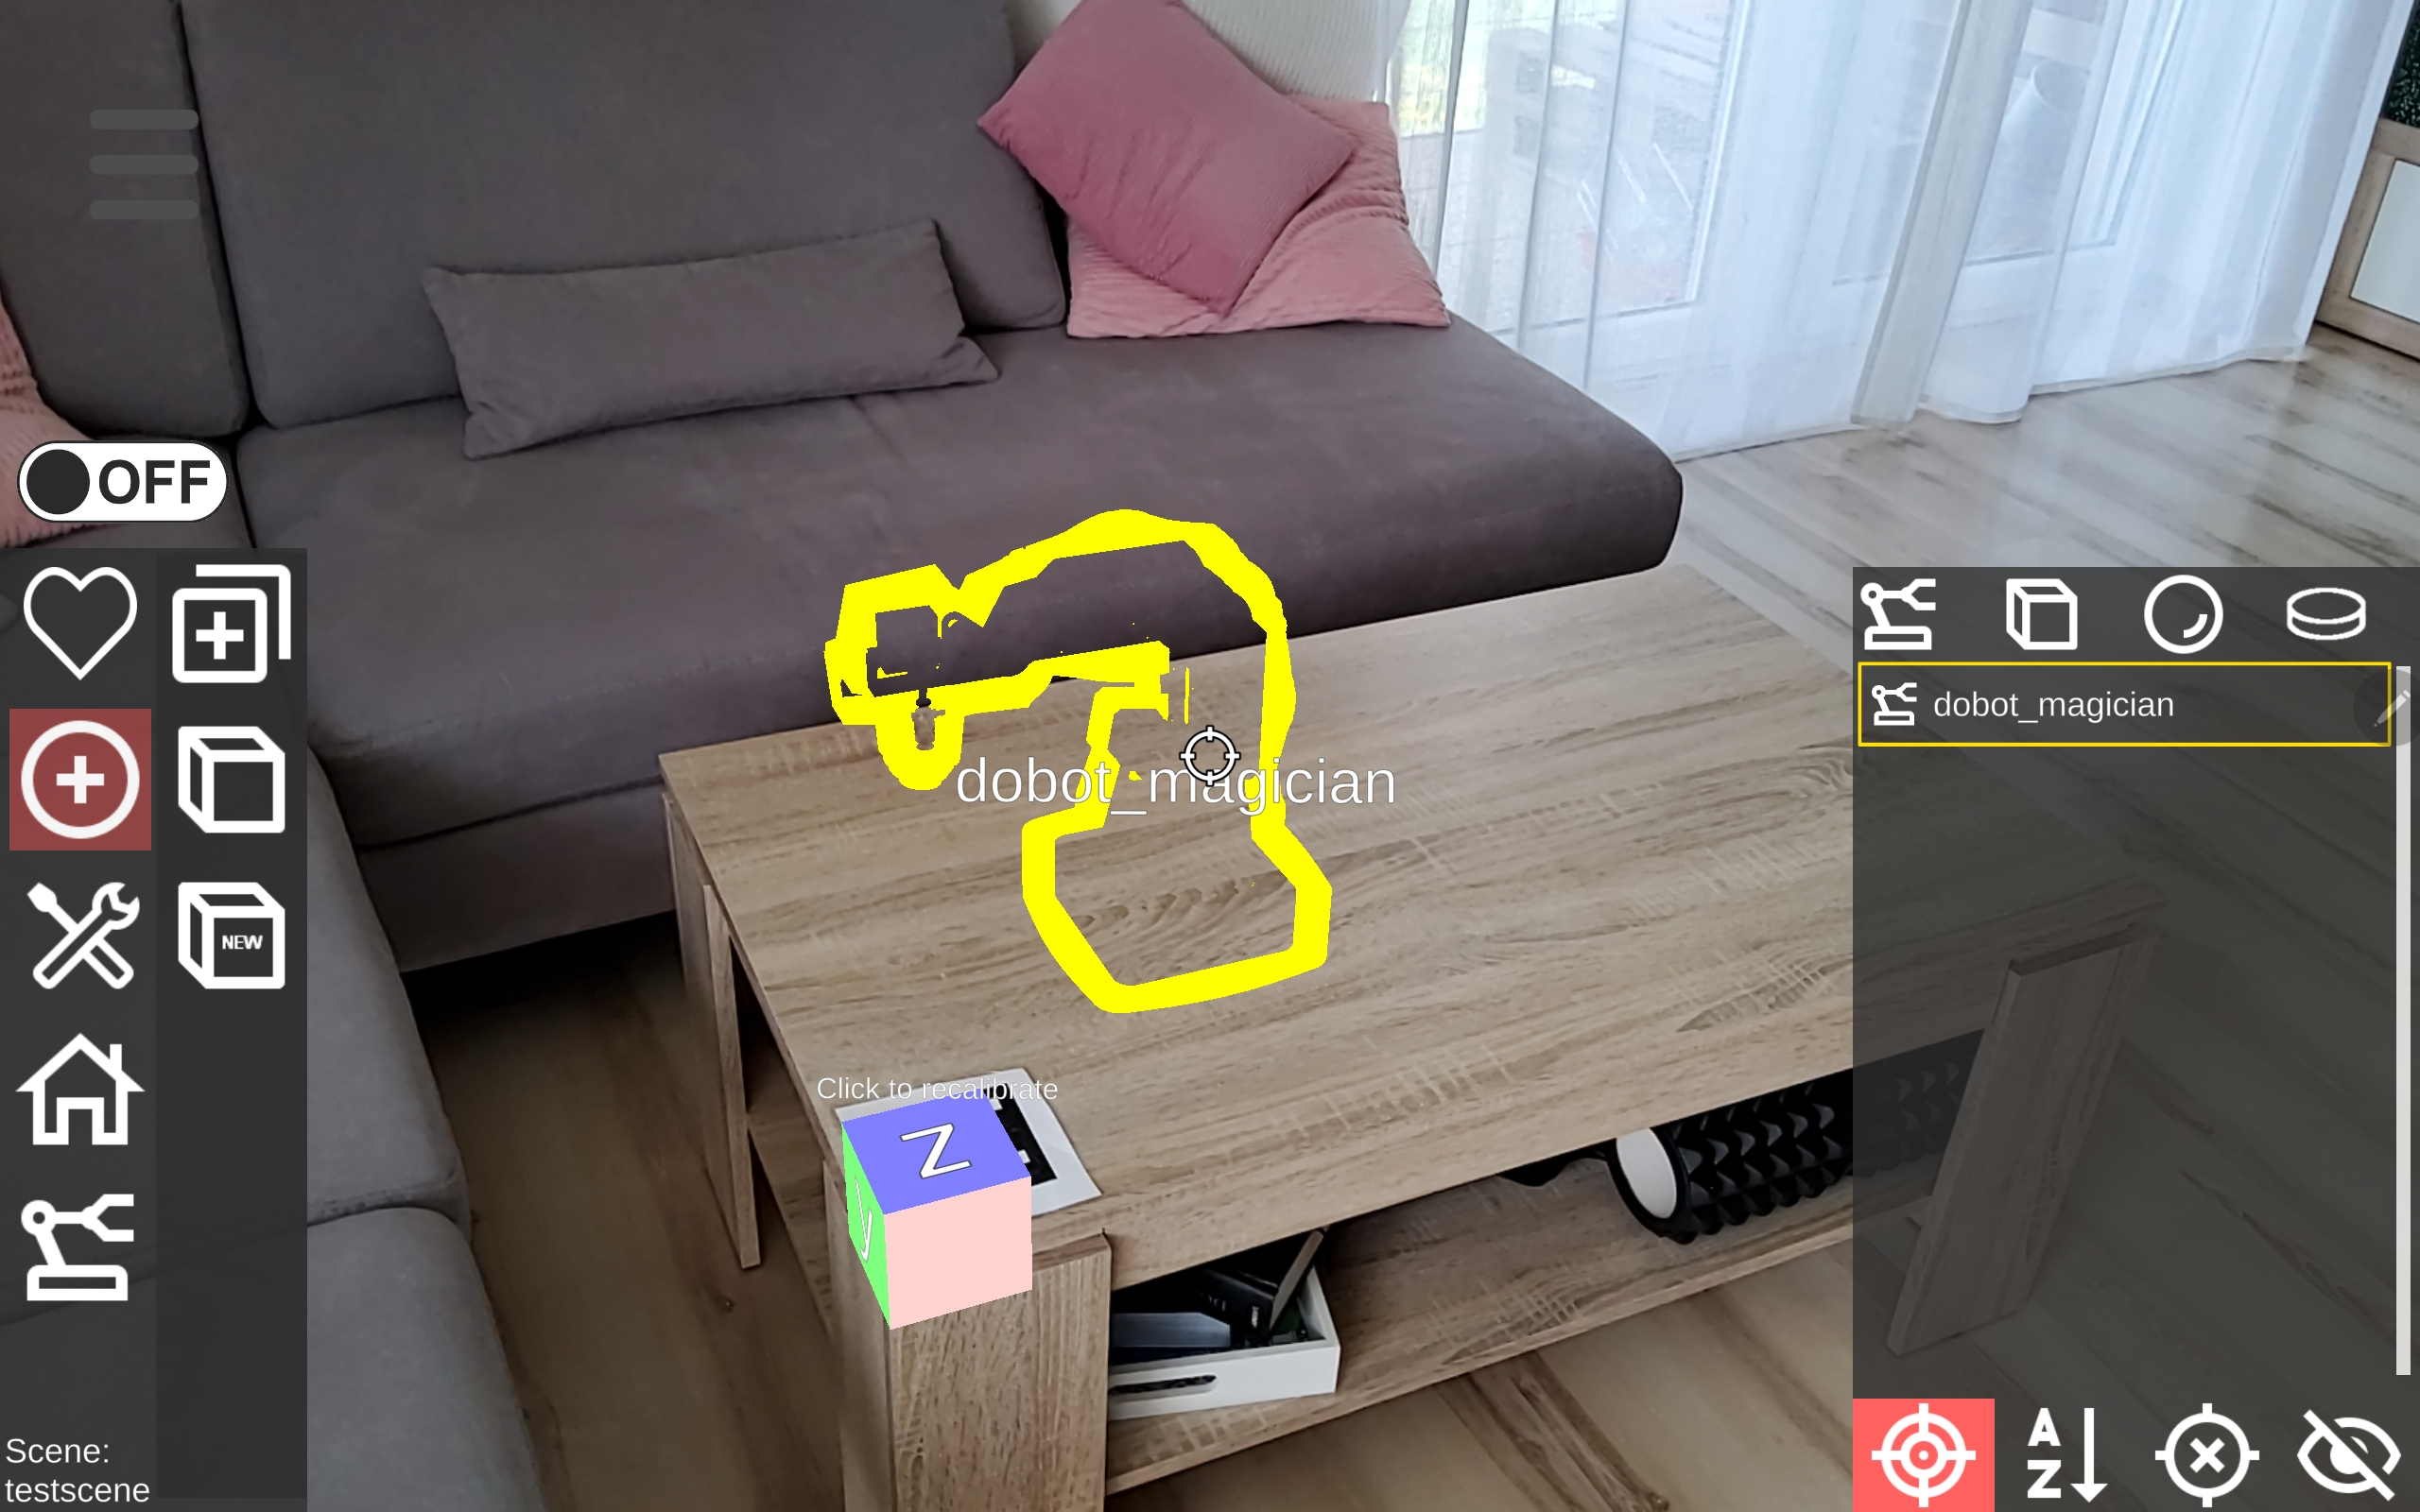
\includegraphics[width=\textwidth]{obrazky-figures/AREditorSelectorMenu.jpg}}
    
        \subfloat['Add object' menu opened.]{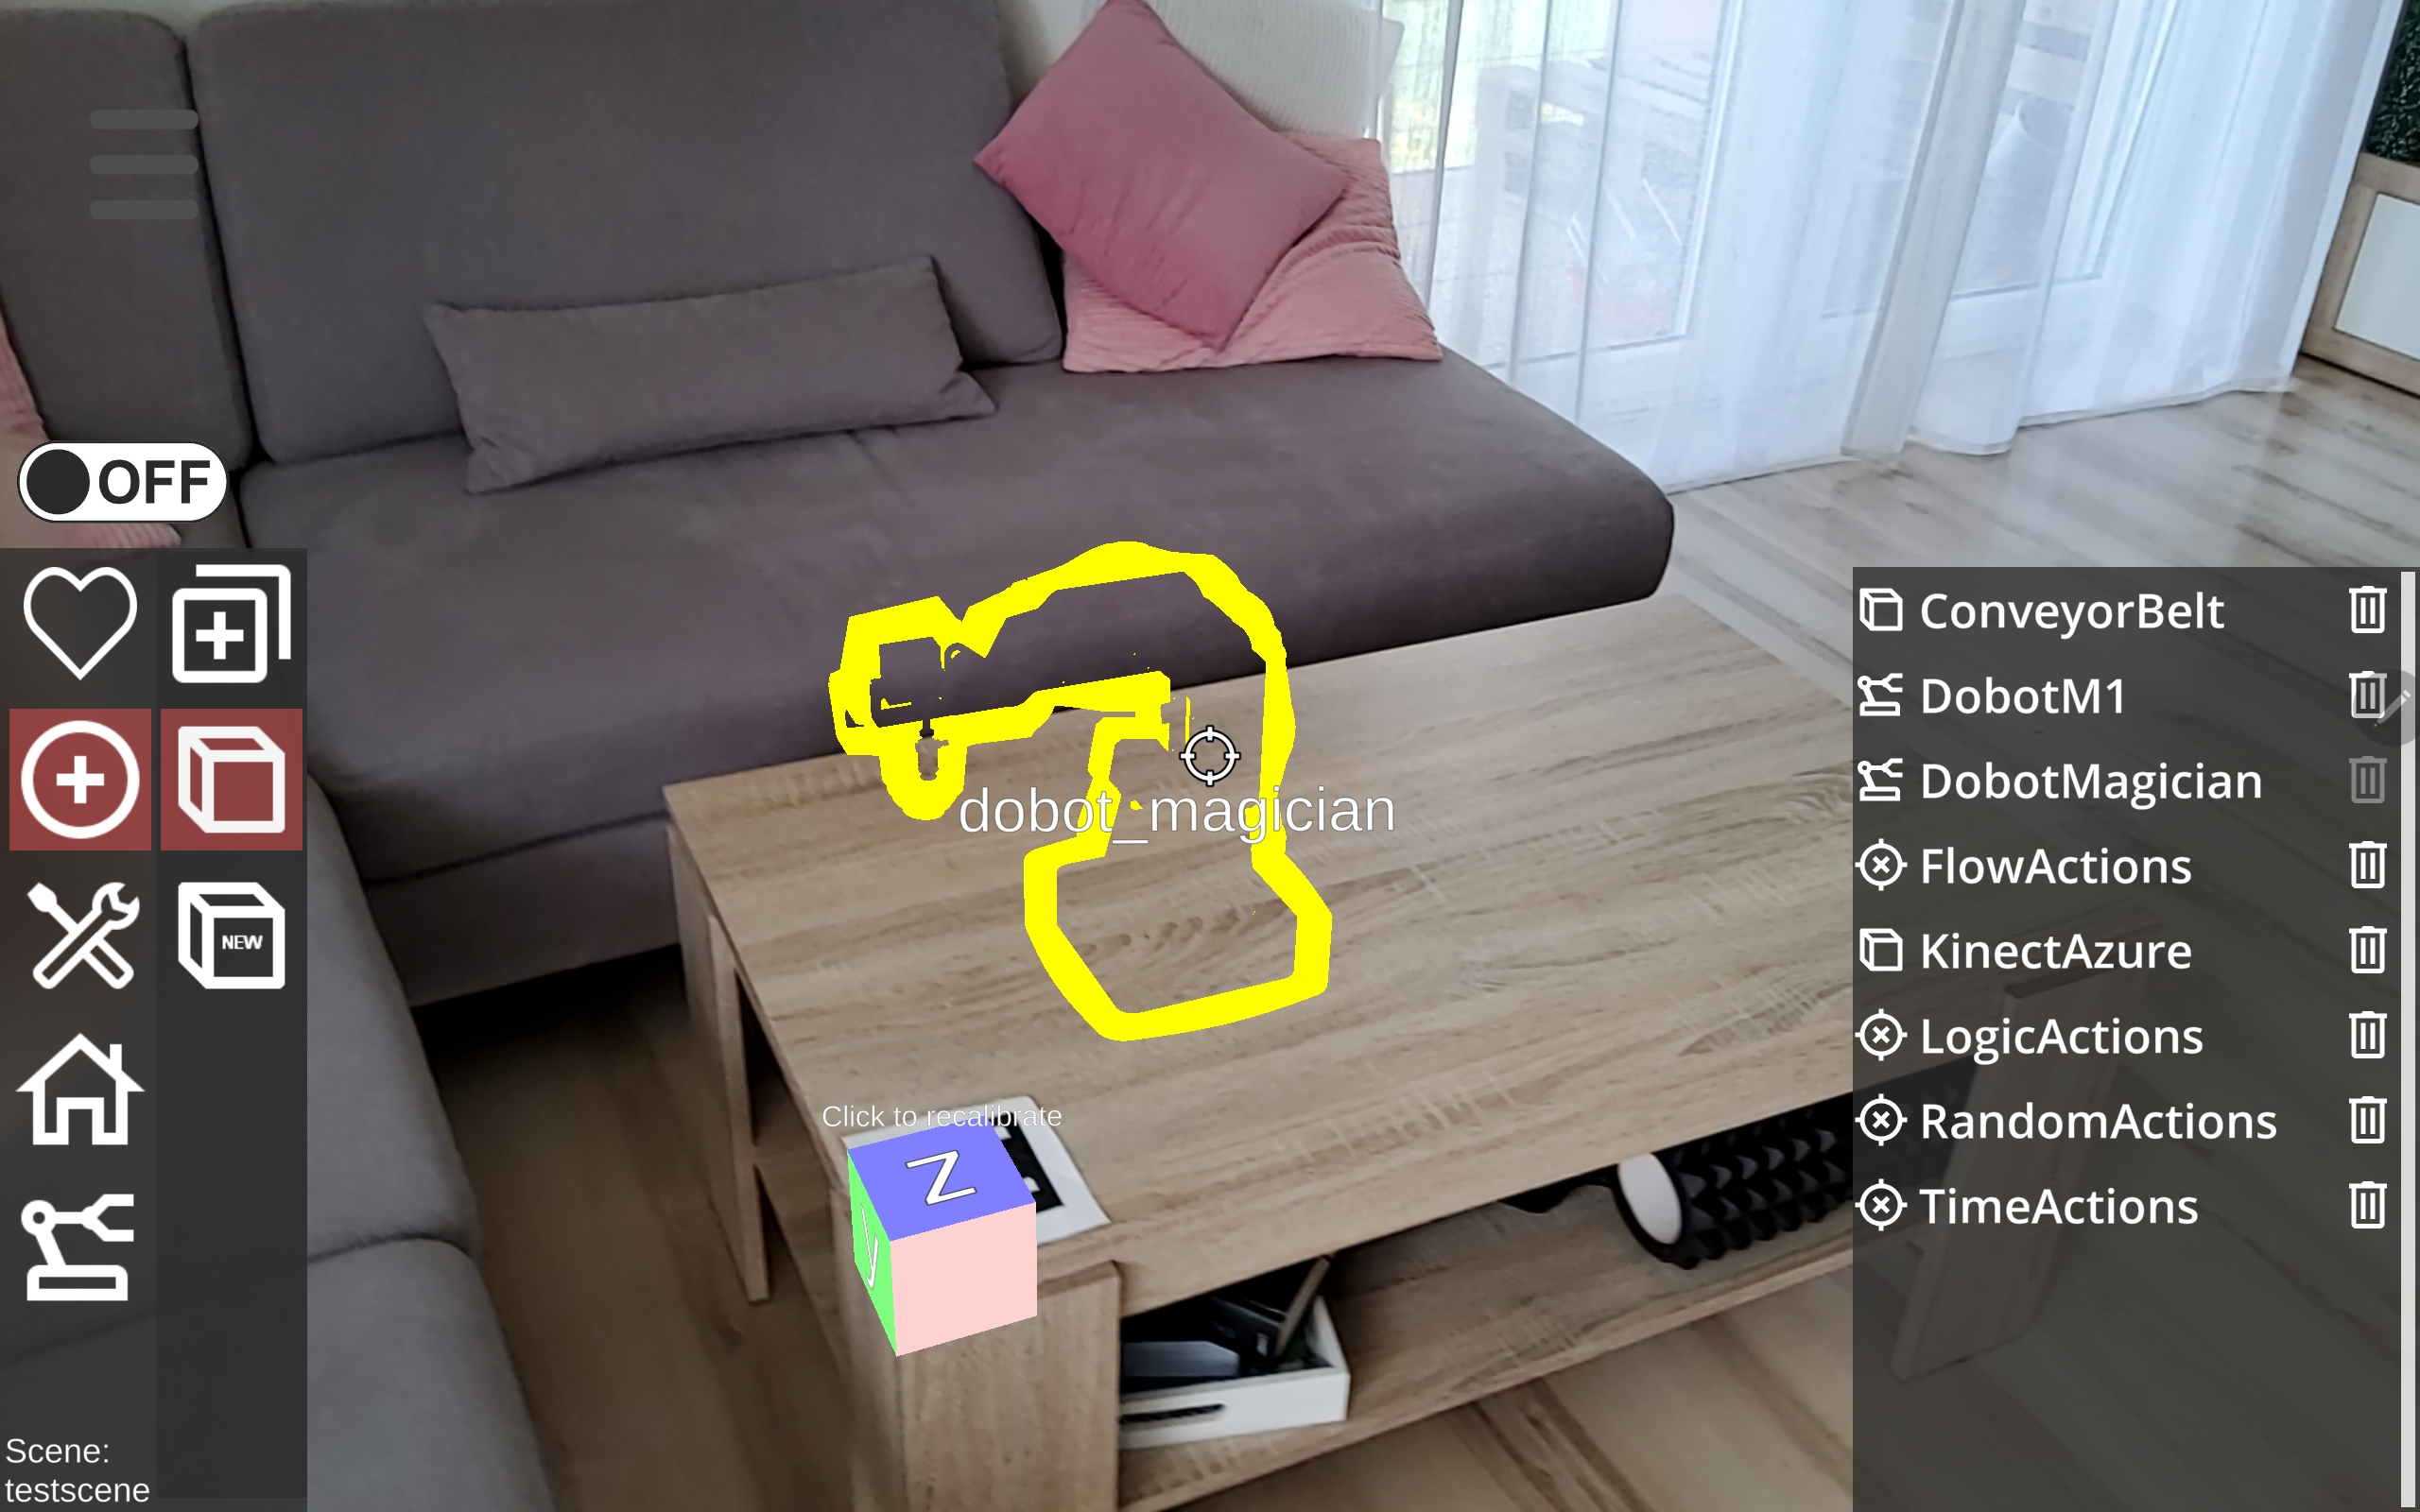
\includegraphics[width=\textwidth]{obrazky-figures/AREditorAddObjectMenu.jpg}}
    
    \caption{Editor screen}
    \label{fig:EditorMenus}
\end{figure}

The editor is designed to be used while holding a tablet with two hands. This approach introduces some limitations but helps prevent fatigue, often present when holding a tablet with a single hand for prolonged periods. Widgets are located on either side of the screen to allow for good visibility of the workspace, as well as to make the individual buttons accessible by thumbs.  

\subsubsection{3D sight}
The sight works as a de facto cursor. It is located in the middle of the screen and is the main interaction method between the user and action objects. AREditor perpetually casts a ray from the center forward and checks for collisions with action objects in the scene. By aiming the crosshair at an action object, the object is highlighted in the selector menu, as well as outlined, as seen in \ref{fig:EditorMenus}. When using the stepping menu or the object manipulation menu, the crosshair is used to select the axis of movement. 

\subsubsection{Object manipulation menu}
An action object can be moved, scaled, or rotated using the object manipulation menu. When the menu is active, a three-axis gizmo appears. By pointing the sight at a particular axis, it becomes selected, after which the transform wheel can be used to move (rotate, scale) the object along said axis. The user can also select the unit of the transform wheel, as well as move the object freely by holding the 'hand' icon and moving the tablet. The menu also offers undo and redo capabilities.


\subsubsection{Robot stepping menu}
The robot stepping menu is the main way of manually setting the pose of a robot within AREditor. The appearance of the menu is similar to object manipulation menu, but the transform wheel is replaced by plus and minus buttons for incremental movement. By stepping the robot, the end-effector is moved in the chosen direction by the selected unit. 

Robot stepping menu also offers two more toggles, a safe/unsafe movement switch and a global/local space switch. Unlike object manipulation menu, scaling option is omitted. Both menus can be seen in \ref{manipulationandstepping}.

\begin{figure}
    \centering
    \subfloat[Object manipulation menu]{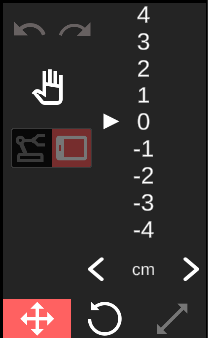
\includegraphics{obrazky-figures/objectmanipulationmenu.png}}\quad
    \subfloat[Robot stepping menu]{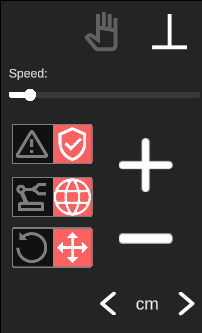
\includegraphics{obrazky-figures/robotsteppingmenu.png}}
    \caption{Object manipulation and robot stepping menus.}
    \label{manipulationandstepping}
\end{figure}

\chapter{Design}
In this chapter, I will go over the design requirements for the proposed system, and the individual parts of the final design.

When programming robots using the ARCOR2 system, a user typically sets action points at the position of the end-effector. An action point is a spatially anchored container, that holds a position and orientation. Actions can then be assigned to action points and program flow is created. The user, therefore, needs to be able to quickly and easily position the robot end-effector to the applicable point in space so that they can set an action point. Furthermore, AREditor is designed to be used with thumbs only, warranting a simple user interface with a limited amount of buttons. 

In most previous works on mobile devices, explicit pose setting of a robot was resolved using on-screen arrows. While this approach works and was briefly considered, a better solution exists. In AREditor, selecting (and moving) objects is already done by utilizing rays cast from the camera, aimed at a chosen object within the scene. This principle can be applied to robot positioning, as described in the next section.

A goal of this design was to provide flexibility while not obscuring the screen space. This is a problem often seen in mobile AR interfaces. Another aim was to make the movement feel natural and easy to learn, making it accessible to end-users of varied levels of experience with tablets or robotics.

\section{Movement}
Two approaches to robot pose setting were considered: moving individual joints, and moving the end-effector only (utilizing inverse kinematics). The first approach was deemed unnecessary, as it's rarely needed. In the vast majority of use-cases, only setting only the end-effector position is sufficient. Secondly, as seen in \cite{Zhang2020AugmentedRI} or \cite{Tango}, this could result in a high number of buttons, obscuring the screen and complicating usage.

By shifting focus from individual joints to the end-effector, the problem can be reduced to a simple point moving in 3D space, and axes can be drawn from the end-effector to facilitate movement in all directions. Early designs featured arrows or joysticks on-screen to be used to move the end-effector along the selected axis (\ref{fig:EarlyDesigns}).



The interface can further be simplified by utilizing augmented reality and tablet movement. After having selected the axis, the object can be simply moved by moving the tablet. The second iteration featured a single button for axis selection and arrows (joysticks) were abandoned \ref{fig:EarlyDesigns2} \subref{SelectableAxes}. This approach also allows for unconstrained movement, which can be used by selecting the end-effector itself, instead of one of the axes. This feature is available by selecting the end-effector itself \ref{fig:EarlyDesigns2} \subref{SelectableEE}. Furthermore, inspired by 3D software such as Fusion 360\footnote{\href{https://www.autodesk.com/products/fusion-360/}{https://www.autodesk.com/products/fusion-360/}} or Godot Engine\footnote{\href{https://godotengine.org/}{https://godotengine.org/}}, the gizmo was modified to include planes, which allow unconstrained movement in a 2-dimensional space. 

\begin{figure}[H]
    \centering
        \subfloat[Design with two sets of joysticks, to control all three axes.]{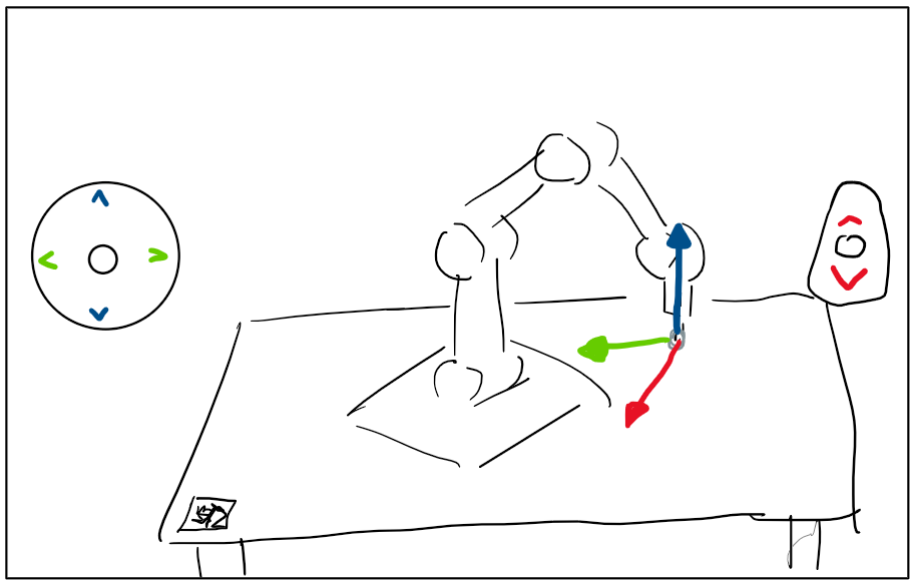
\includegraphics[width=0.8\textwidth]{obrazky-figures/EarlyDesign2.png}
        \label{EarlyDesign2}}
    
        \subfloat[Arrows replace joysticks, and a dial to set the gizmo rotation.]{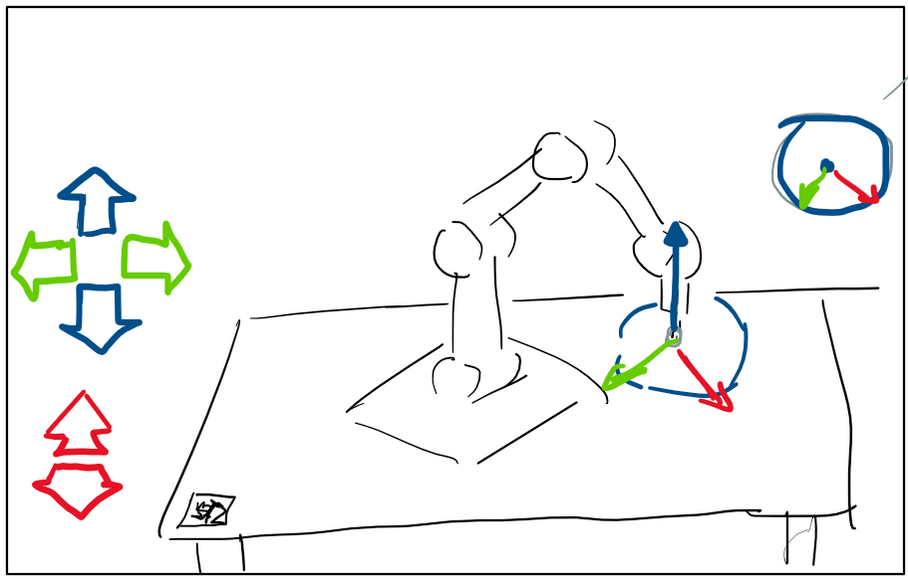
\includegraphics[width=0.8\textwidth]{obrazky-figures/EarlyDesign1.png}
        \label{EarlyDesign1}}
    
    \caption{Early designs with on-screen touch controls}
    \label{fig:EarlyDesigns}
\end{figure}

\begin{figure}[H]
    \centering
        \subfloat[Selectable axes]
        {
        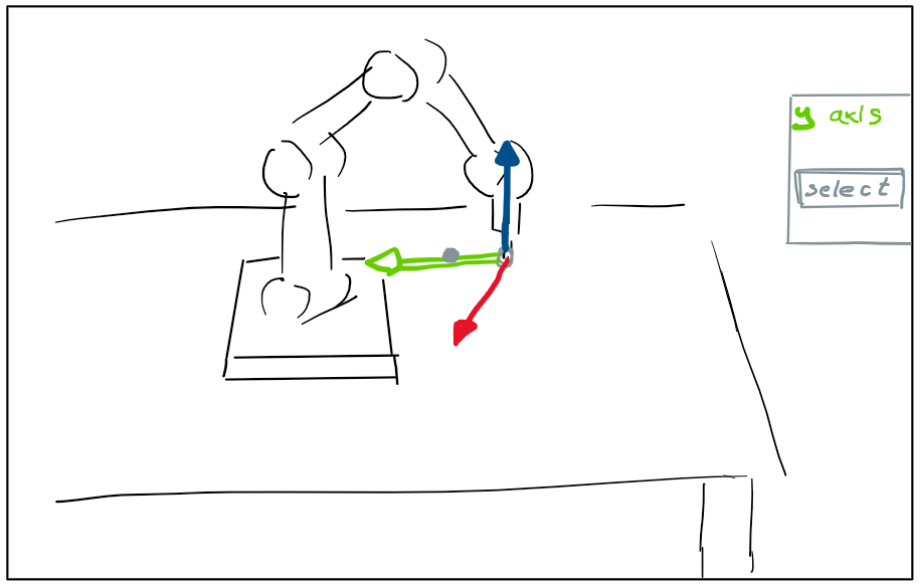
\includegraphics[width=0.8\textwidth]{obrazky-figures/EarlyDesign3.png}
        \label{SelectableAxes}
        }
    
        \subfloat[Selectable end-effector]{
        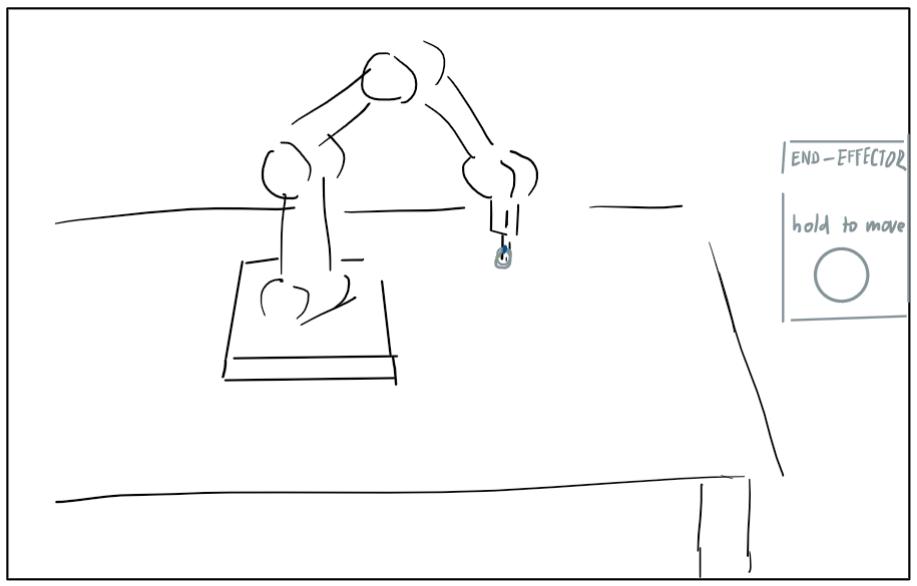
\includegraphics[width=0.8\textwidth]{obrazky-figures/EarlyDesign4.png}
        \label{SelectableEE}
        }
    
    \caption{Design variants employing tablet movement. These were later combined into singular design.}
    \label{fig:EarlyDesigns2}
\end{figure}

\subsection{Forward/backward buttons}

To facilitate movement in the direction from the user to the robot, an additional control was added. To move the end-effector forwards, one would have to move the tablet forwards the same amount, which proved to be impractical. In order to allow the operator to keep the same distance from the robot throughout the session, a different way to move the end effector along said axis was neccessary. A dual button control was added, featuring slanted arrow icons to illustrate forward/backward direction of movement (\ref{fig:forwardbackwardbuttons}). 

These buttons were later modified to only affect the horizontal plane, ignoring the vertical axis. This was decided after a consultation, where it was deemed to be the more logical approach. The buttons were added to remove the need to walk forward and backward, regardless of the height of the user. \myworries{add a picture perhaps}
\\
\begin{figure}[H]
    \centering
    
\includegraphics{obrazky-figures/forwardbackwardbuttons.png}
    \caption{Forward/backward buttons.}
    \label{fig:forwardbackwardbuttons}
\end{figure}

\subsection{Sensitivity sliders}

When dragging the end-effector, the end-effector position moves to the exact position of the raycast at a specified distance. This is the most intuitive outcome, but standing farther away, the same tablet movement results in a larger robot movement. For example, when standing 1.5 meters away and rotating the tablet by 15\degree, while having the X axis selected, the end-effector will move by 40 centimeters. If the operator stood a meter farther, the end-effector would move by 66 centimeters. This scenario is illustrated in \ref{fig:closefar}. For more precise positioning at farther distances, the option to lower the sensitivity was introduced. The slider value acts as a distance multiplier and is by default set to 1, which moves the end-effector to the exact final raycast hit and can be lowered to shorten the distance traveled by the robot arm. 

Similarly, a slider for the forward/backward buttons was added, to control the speed of the movement. 

\begin{figure}
    \centering
    \subfloat{
        \includesvg[width=0.3\textwidth]{obrazky-figures/dobotmagician.svg}
        \label{close}
    }
    \qquad
    \subfloat{
        \includesvg[width=0.3\textwidth]{obrazky-figures/dobotmagicianfar2.svg}
        \label{far}
    }
    
    \caption{The same tablet rotation from different distances.}
    \label{fig:closefar}
\end{figure}

\subsection{User-relative coordinate system}

To allow the user to move the end-effector along arbitrary axis in the horizontal plane, two approaches were examined. Initially, a dial for manually rotating the gizmo around its vertical axis was considered (\ref{fig:EarlyDesigns}\subref{EarlyDesign1}). A more intuitive approach is to make the gizmo rotation relative to the tablet position. In this scenario, the gizmo rotates as the user moves around the workplace, with one axis staying perpendicular to the camera position and the second one oriented towards the camera position \myworries{pic}. Another addition is a lock button, which allows the operator to lock the current gizmo rotation. This system enables movement along arbitrary axes, which can be aligned with other objects in the workplace by simply walking toward them while maintaining the repeatability of movements provided by the lock button. 

\section{User interface}
The system consists of several separate submenus: the main menu, forward/backward buttons, and a confirmation dialog.

The main menu's central component is the select button. It also contains a label indicating the current selection, a sensitivity slider, and the coordinate system switch. The select button has a description label "hold to drag", which gets hidden when dragging. The coordinate system switch has two switchable states, \textit{world} and \textit{user}, through which the user-relative coordinate system can be enabled. When the \textit{user} state is selected, the lock button appears. 

The layout follows previously established conventions in AREditor. The main menu is located on the right side of the screen, with the confirmation dialog beneath. The main menu is also the only menu, that is always visible. If the pose of the robot model is the same as the real robot, the confirmation dialog is not visible. It only appears, when a movement robot model is executed, and is only enabled, when the user concludes the movement. The confirmation dialog contains two buttons, \textit{apply} and \textit{revert}, through which the operator can send the pose to be applied to the real robot, or revert the model to the default state (copy the pose of the real robot). Additionally, while dragging, the left menu along with the online/offline switch are hidden. The layout of the menus can be seen in \ref{fig:layout}.

\begin{figure}
    \centering
    \subfloat[The layout when not moving.]{
        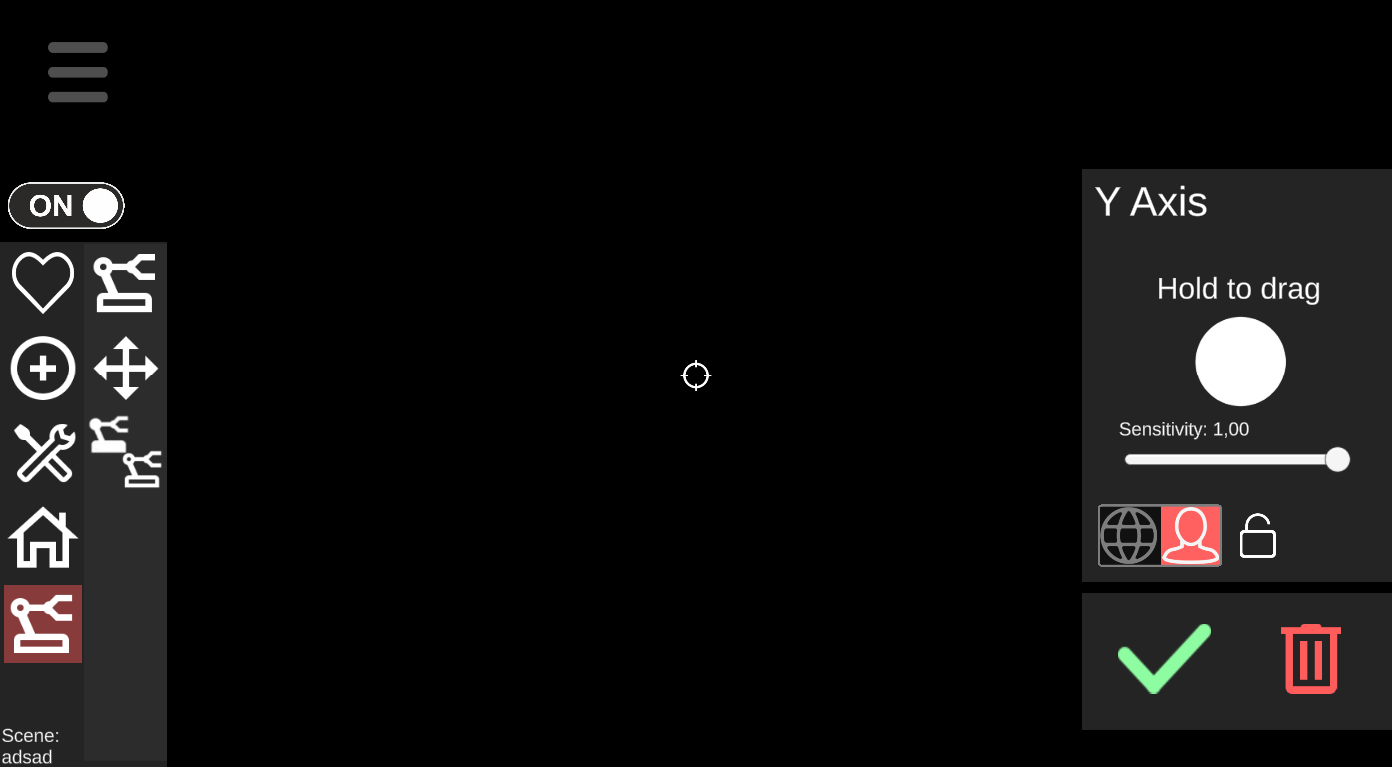
\includegraphics[width=0.8\textwidth]{obrazky-figures/Layout.png}
        \label{notmoving}
    }
    \\
    \subfloat[The layout when moving the end-effector.]{
        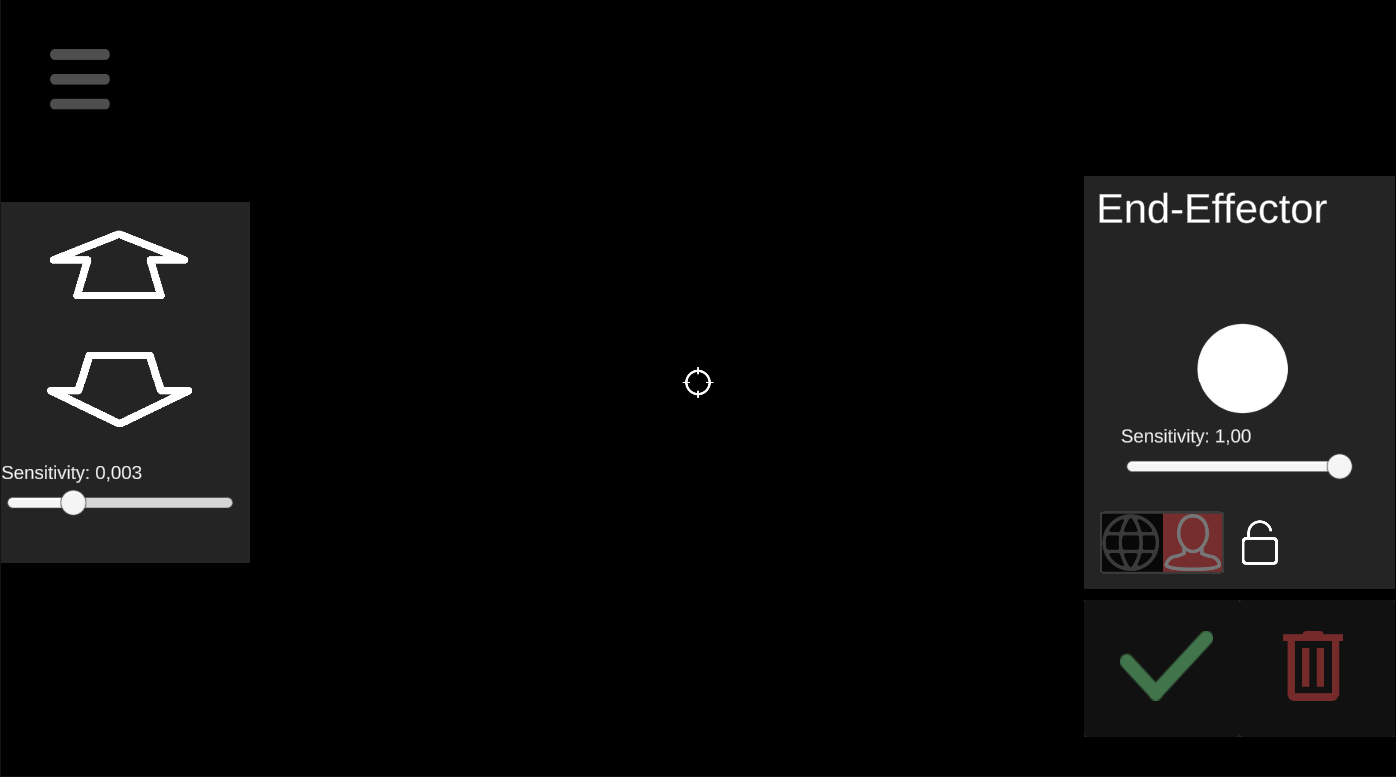
\includegraphics[width=0.8\textwidth]{obrazky-figures/LayoutWhenMoving.png}
        \label{moving}
    }
    
    \caption{A comparison of the old notification and the new notification.}
    \label{fig:layout}
\end{figure}

\subsection{Invalid pose indication} 
\myworries{should this be under User interface, or a separate section?}

To inform the user that the pose is out of bounds, visual indicators were included in the design. The original notification system was insufficient for the purposes of this solution for two reasons: readability and performance, the first of which will be characterized in this section. Performance is discussed in the \textit{Implementation} chapter.

Notifications in the original notification system are implemented as temporary messages in the top right corner of the screen. A notification is presented in the form of a semi-transparent grey box, which contains text. If the notification is informing of a failed RPC request, it usually contains a title and the error message from ARServer. The notification fades in, is displayed for a brief period, and then fades out. 

This work entails a different form of notification. The user has to be notified exactly when an impossible pose is reached, and vice versa, when the point is back in a valid position, for quicker understanding of the current state. The message should also be simpler, as there is no need to display the full RPC response message.

The new notification is a red box, containing the text "Invalid pose" written in large, white text. The RPC response message was removed. It appears immediately after the user moves the end-effector beyond the reach of the robot, and is hidden once the end-effector is back in the work envelope of the robot arm. A comparison between the old and the new notifications can be seen in \ref{fig:notifications}.

\begin{figure}[h]
    \centering
    \subfloat[The old notification.]{
        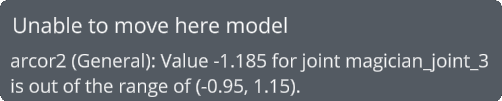
\includegraphics{obrazky-figures/OldNotification.png}
        \label{old}
    }
    \\
    \subfloat[The new notification.]{
        
\includegraphics{obrazky-figures/ImpossiblePoseNotification.png}
        \label{new}
    }
    
    \caption{A comparison of the old notification and the new notification.}
    \label{fig:notifications}
\end{figure}

An additional visual cue was added to further indicate, that the robot is in an unreachable pose. Upon leaving the work envelope, the robot model is displayed in red \myworries{img}. A more elaborate, albeit similar approach was taken in \cite{ONG2020101820}, Where the overlaid robot model arm is displayed in colors from green to red, based on the manipulability of the robot. The system calculates manipulability based on a scale proposed by Yoshikawa \cite{yoshikawa}. In the ARCOR2 system, no such manipulability scale is implemented and is out of the scope of this work, therefore a simpler, yet still effective, approach was chosen.

\chapter{Implementation}

The system was integrated into AREditor as a new menu in the 'Robot' category. The entire solution is contained within one prefab, with the class \texttt{ModelSteppingMenu} attached. 

\chapter{Testing}
\begin{itemize}
    \item moderated
    \item in-person
    \item assessment/comparative?
\end{itemize}

Questionaire:
\begin{itemize}
    \item Experience with tablet
    \item Experience with AR
    \item Experience with 3D apps (Blender/Fusion 360/other)
    \item Other questions?
\end{itemize}

Scenario:
\begin{itemize}
    \item There will be a target point (action point) in the scene
    \item Users will move the robot to that point using the \emph{model stepping menu}
    \item Users will then move the robot to that point using the \emph{robot stepping menu} (might not be neccessary in case of assessment testing only)
    \item Time to reach the final point will be measured (times will be compared)
    \item Users' choice of movement (free/axis/plane) will be noted
    \item Users' sensitivity setting will be noted
    \item Users' use of forward/backward buttons will be noted
\end{itemize}



\chapter{Conclusion}